\section{Procedimento \& Analisi dati}

\subsection{Relazione tra indice di rifrazione e lunghezza d'onda}

La prima operazione eseguita è stata quella di misurare l'angolo ``zero''. Ovvero abbiamo misurato l'angolo segnato dal goniometro quando tra la sorgente luminosa e il canocchiale, allineati, non vi era interposto alcun'oggetto. Ricordiamo che più si stringe la fenditura del collimatore più la misura dell'angolo ``zero'' risulta essere precisa, tuttavia stringendo troppo non si vede una mazza. Bisogna quindi arrivare ad un compromesso.
L'angolo ``zero'' quindi ha il seguente valore:

\begin{equation}
	\theta\ped{0} \,=\, 128^\circ \,31' \pm 1'
\end{equation} 
%
dove abbiamo considerato l'incertezza di risoluzione pari ad un primo anche se il goniometro ha una risoluazione di misura di 30''.

Ora vogliamo osservare la relazione che sussiste tra l'indice di rifrazione del nostro prisma di vetro e la lunghezza d'onda di un raggio luminoso.
A tal fine occorre ricordare che un raggio luminoso incidente su una faccia di un prisma subisce una riflessione e una rifrazione, poichè passa da un mezzo ad un altro.
Consideriamo ora cosa accade al raggio rifratto. Poichè il raggio luminoso incidente non è monocromatico questo è composto da numerosi raggi luminosi con lunghezza d'onda differente, in base alla sorgente che emette i raggi. Quando il raggio incidente viaggia attraverso il prisma si scompone nelle sue varie componenti (dispersione della luce) a seconda delle diffrenti lunghezze d'onda che lo compongono. Quindi i raggi monocromatici subiscono un'ulteriore rifrazione passando nuovamente dal vetro all'aria, uscendo infine dal prisma. Questa seconda rifrazione non porta altro che ad un'amplificazione dell'effetto precedente, pertanto è più semplice distinguere i vari raggi luminosi.

In questa esperienza noi non siamo in grado di misurare direttamente la lunghezza d'onda di un raggio luminoso. Per superare questo ostacolo si può sfruttare una lampada a gas, che ha la particolarità di emettere luce solo a determinate lunghezze d'onda, in base al tipo di gas nella lampada. Scomponendo con il prisma la luce proveniente dalla lampada a gas (nel nostro caso una lampada al cadmio), si possono osservare i raggi corrispondenti alle lunghezze d'onda che essa emette.

Note a priori le lunghezze d'onda, si può ottenere il valore dell'indice di rifrazione per una specifica lunghezza d'onda misurando l'algolo di deviazione $\theta\ped{max}$, ovvero l'angolo formato dai prolungamenti dei raggi incidente e di uscita dal prisma (si veda Figura \ref{fig:prisma} per maggiore chiarezza).

Il calcolo si semplifica notevolmente se si adotta la seguente strategia. L'angolo di deviazione $\theta\ped{max}$ varia al variare dell'angolo di incidenza. Si può dimostrare, sia sperimentalmente che teoricamente, che esiste un angolo massimo di deviazione che corrisponde alla configurazione in Figura \ref{fig:prisma}. Si può notare che la configurazione è simmetrica, ovvero l'angolo di incidenza $\theta_i$ è uguale all'angolo di uscita (rispetto alla normale alla superficie). Con semplici considerazioni geometriche, conoscendo l'angolo massimo $\theta\ped{max}$ di deviazione, si può ricavare l'indice di rifrazione del prisma con la seguente relazione:

\begin{SCfigure}[0.6][t]
    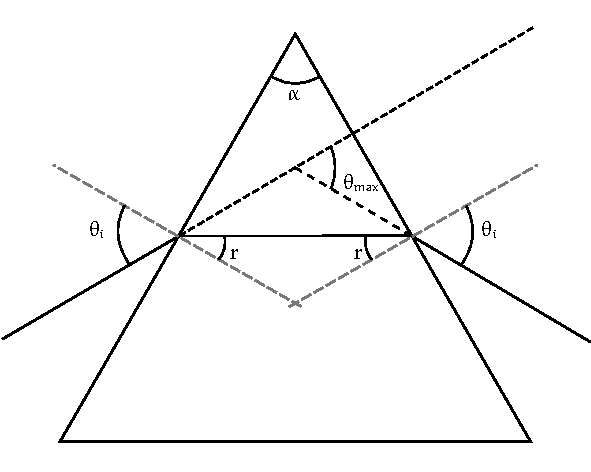
\includegraphics[width=10cm]{prisma1.pdf}
    \caption{}
    \label{fig:prisma}
\end{SCfigure}

\begin{equation}
	n \,=\, \frac{\sin{(\frac{\alpha \,+\, \theta\ped{max}}{2})}}{\sin{\frac{\alpha}{2}}}
	\label{indice_rif}
\end{equation}

dove $\alpha$ è l'angolo di apertura del prisma (vedi Figura \ref{fig:prisma}), che nel nostro caso vale $60^\circ$.

Questa è la teoria che sta alla base dell'esperienza. Operativamente per misurare $\theta\ped{max}$ abbiamo adottato la seguente procedura:

\begin{itemize}
	\item{Si posiziona il prisma al centro del goniometro. Successivamente si ruota il prisma per cercare di ottenere $\theta\ped{max}$, aiutandosi con il canocchiale. $\theta\ped{max}$ si ottiene quando, continuando ad aumentare l'angolo di incidenza, l'angolo di deviazione si ferma e ``torna indietro'';}
	\item{Una volta ottenuto $\theta\ped{max}$ si allinea il canocchiale col crocefilo con il raggio monocromatico in esame e si legge sullo spettrogoniometro il valore dell'angolo segnato $\theta\ped{\lambda}$, dove $\lambda$ sta per la lunghezza d'onda del raggio;}
	\item{Quindi per ottenere $\theta\ped{max,\lambda}$ non si deve fare altro che una semplice differenza tra $\theta\ped{\lambda}$ e $\theta\ped{0}$;}
\end{itemize}

Infine una volta ottenuti i vari valori di $\theta\ped{max,\lambda}$, uno per ciascuno dei raggi monocromatici che siamo stati in grado di distinguere, ne calcoliamo il rispettivo indice di rifrazione sfruttando la relazione (\ref{indice_rif}). I valori che abbiamo ottenuto sono riportati nella seguente tabella (Tabella \ref{tab:enne}), nella quale è stato associato al colore del raggio monocromatico la rispettiva lunghezza d'onda.

\begin{table}[H]
    \centering
    \small
    \begin{tabular}{l c c}
        \toprule
        Colore & $\theta\ped{max}$ & $n \pm dn$ \\
        \midrule
		Rosso 1	& 	$167^\circ \, 00' \pm 1'$ &	$1.5149 \pm 0.0003$ \\	
		Rosso 2	& 	$167^\circ \, 02' \pm 1'$ &	$1.5153 \pm 0.0003$ \\
		Rosso 3	& 	$167^\circ \, 05' \pm 1'$ &	$1.5159 \pm 0.0003$ \\
		Verde &		$167^\circ \, 32' \pm 1'$ &	$1.5210 \pm 0.0003$ \\
		Blu &		$167^\circ \, 42' \pm 1'$ &	$1.5229 \pm 0.0003$ \\
		Viola &		$167^\circ \, 47' \pm 1'$ &	$1.5238 \pm 0.0003$ \\
        \bottomrule
    \end{tabular}
    \caption{Dati relativi all'indice di rifrazioe $n$ in funzione del colore e quindi della lunghezza d'onda $\lambda$.}
    \label{tab:enne}
\end{table}


\begin{figure}[t]
    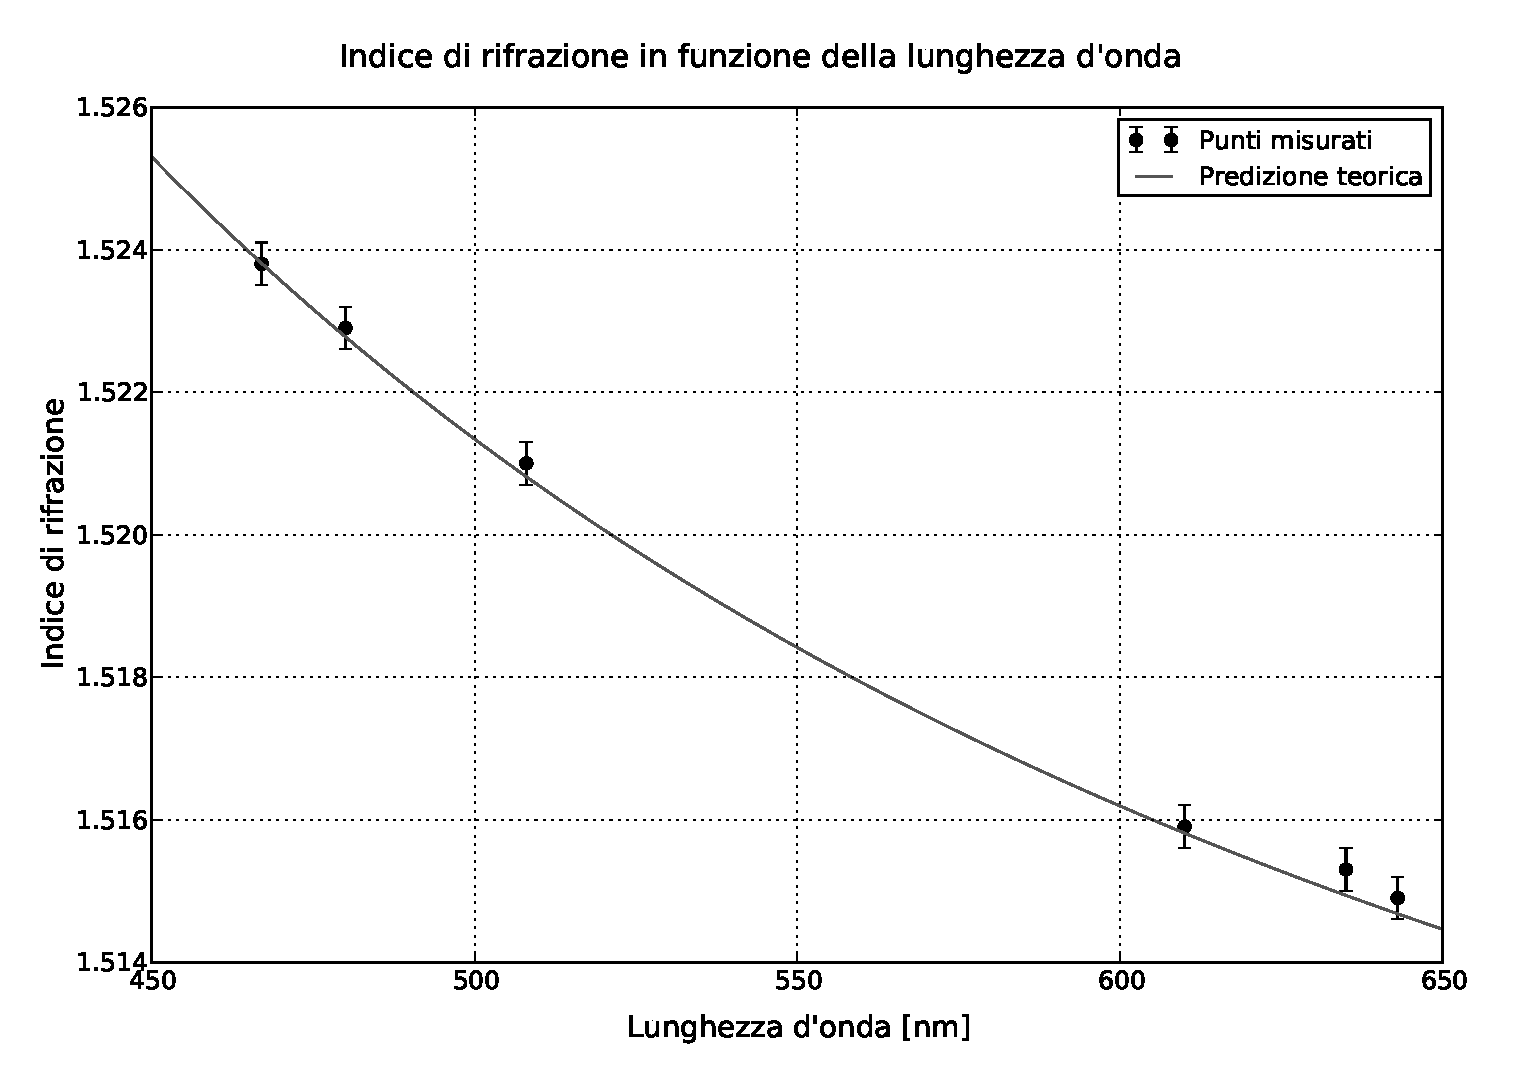
\includegraphics[width=16cm]{wave_index.pdf}
    \caption{}
    \label{fig:prisma}
\end{figure}

Come possiamo notare dai valori tabulati, l'indice di rifrazione per la luce di colore verde, blu e viola varia solo se si osserva la terza cifra decimale, mentre per le differenti tonalità di rosso occorre quasi la quarta. Invece la differenza tra le sfumature di rosso e i tre colori verde, blu e viola si può notare anche esaminando solo la seconda cifra decimale.

Queste differenze hanno senso perchè, osservando con il canocchiale la distanza tra le righe dei vari colori, il raggio rosso era sensibilmente più distante dagli altri, come si può notare anche dai rispettivi valori di lunghezza d'onda. Il colore rosso si trova ad un estremo dello spettro del visibile, mentre i raggi verde, blu e viola sono più vicini all'altra estremità dello spettro. Sperimentalmente abbiamo avuto non poche difficoltà ad individuare le due gradazioni di rosso oltre a quella primaria (Rosso 1), poiché le rispettive lunghezze d'onda non sono così marcatamente differenti e soprattutto poiché l'intensità del raggio luminoso era particolarmente bassa.
Come già notato gli indici di rifrazione delle tre tonalità di rosso sono molto simili, al punto che i valori sono tra di loro compatibili.

\subsection{Relazione tra angolo di incidenza e di deviazione}

In questa seconda parte dell'esperienza vogliamo verificare la seguente legge. Questa relazione permette di calcolare l'angolo di deviazione di un raggio rispetto alla direzione iniziale, quando questo passa attraverso un prisma.

\begin{equation}
	\theta \,=\, \arcsin{(n - \sin{r})} + \arcsin{(n \, \sin{(\alpha - r)})} - \alpha
	\label{eq:brutta}
\end{equation}
%
dove $n$ indica l'indice di rifrazione del materiale di cui è fatto il prisma, $\theta$ indica l'angolo di deviazione del raggio uscente rispetto al prolungamento del raggio incidente, $\alpha$ non è altro che l'angolo di apertura del prisma, e $r$, rappresenta l'angolo di rifrazione interno al prisma, ovvero l'angolo del raggio rifratto rispetto alla perpendicolare (si veda Figura \ref{fig:prisma}, ricordando che in figura $\theta$ è indicato con $\theta\ped{max}$ e la configurazione in questo caso può non essere simmetrica). L'angolo $r$ si ricava immediatamente dalla legge di Snell:

\begin{equation}
	 n\ped{aria} \, \sin{\theta\ped{i}} = \sin{\theta} = n \, \sin{r}
	 \label{snell}
\end{equation}
%
dove $n\ped{aria}$ rappresenta l'indice di rifrazione dell'aria, che prendiamo uguale a 1, mentre $n$ rappresenta l'indice di rifrazione del materiale di cui è fatto il prisma, che dipende dalla lunghezza d'onda $\lambda$ della luce che colpisce il prisma. Ricordiamo che i valori di $n$ per vari valori di $\lambda$ sono stati ricavati nella prima parte dell'esperienza. Infine $\theta\ped{i}$ rappresenta l'angolo di incidenza del raggio luminoso sulla faccia del prisma.
Quindi usando la (\ref{snell}) e la (\ref{eq:brutta}), è possibile calcolare l'andolo di deviazione $\theta$ in funzione dell'angolo di incidenza $\theta_i$.

Pertanto quello che dobbiamo fare, in pratica, è misurare alcuni valori di $\theta$ e $\theta\ped{i}$, e verificare che siano in accordo con la teoria. Abbiamo seguito il seguente procedimento:

\begin{itemize}
	\item{Abbiamo scelto di ricavare $\theta$ per il raggio monocromatico di colore verde, quindi di lunghezza d'onda pari a 508 nm. Per il calcolo delle formule (\ref{eq:brutta}) e (\ref{snell}) serve infatti l'indice di rifrazione del materiale. Abbiamo scelto di usare la luce verde e quindi il rispettivo valore di $n$ riportato in Tabella \ref{tab:enne};}
	\item{Non potendo misurare direttamente l'angolo di incidenza $\theta\ped{i}$ abbiamo misurato l'angolo di riflessione del raggio riflesso (una componente della luce incidente viene riflessa). Abbiamo mirato con il canocchiale col crocifilo la raggio riflesso, e misurato l'angolo. Quindi sapendo che l'angolo di incidenza non è altro che la metà dell'angolo misurato abbiamo trovato $\theta\ped{i}$;}
	\item{Quindi per ognuno dei 23 angoli di incidenza misurati, abbiamo preso il corrispettivo valore di $\theta$ allineando il canocchiale con il raggio monocromatico verde uscente al prisma;}
	\item{Infine confronteremo i $\theta$ sperimentali con i valori trovati grazie alla relazione (\ref{eq:brutta}) e verificheremo se quest'utima è una relazione valida;}
\end{itemize}

Come si può osservare dal grafico infigura (\ref{fig:dev}) abbimo ottenuto dei datisperimentali che combaciano molto bene con la legge da verificare (\ref{eq:brutta}). Tralasciando due punti, che con molta probabilità non sono stati presi accuratamente come gli altri ci sentiamo di dire che la relazione (\ref{eq:brutta}) che lega $\theta$ con l'angolo di incidenza del raggio luminoso sulla faccia del prisma è verificata.

\begin{figure}[b]
    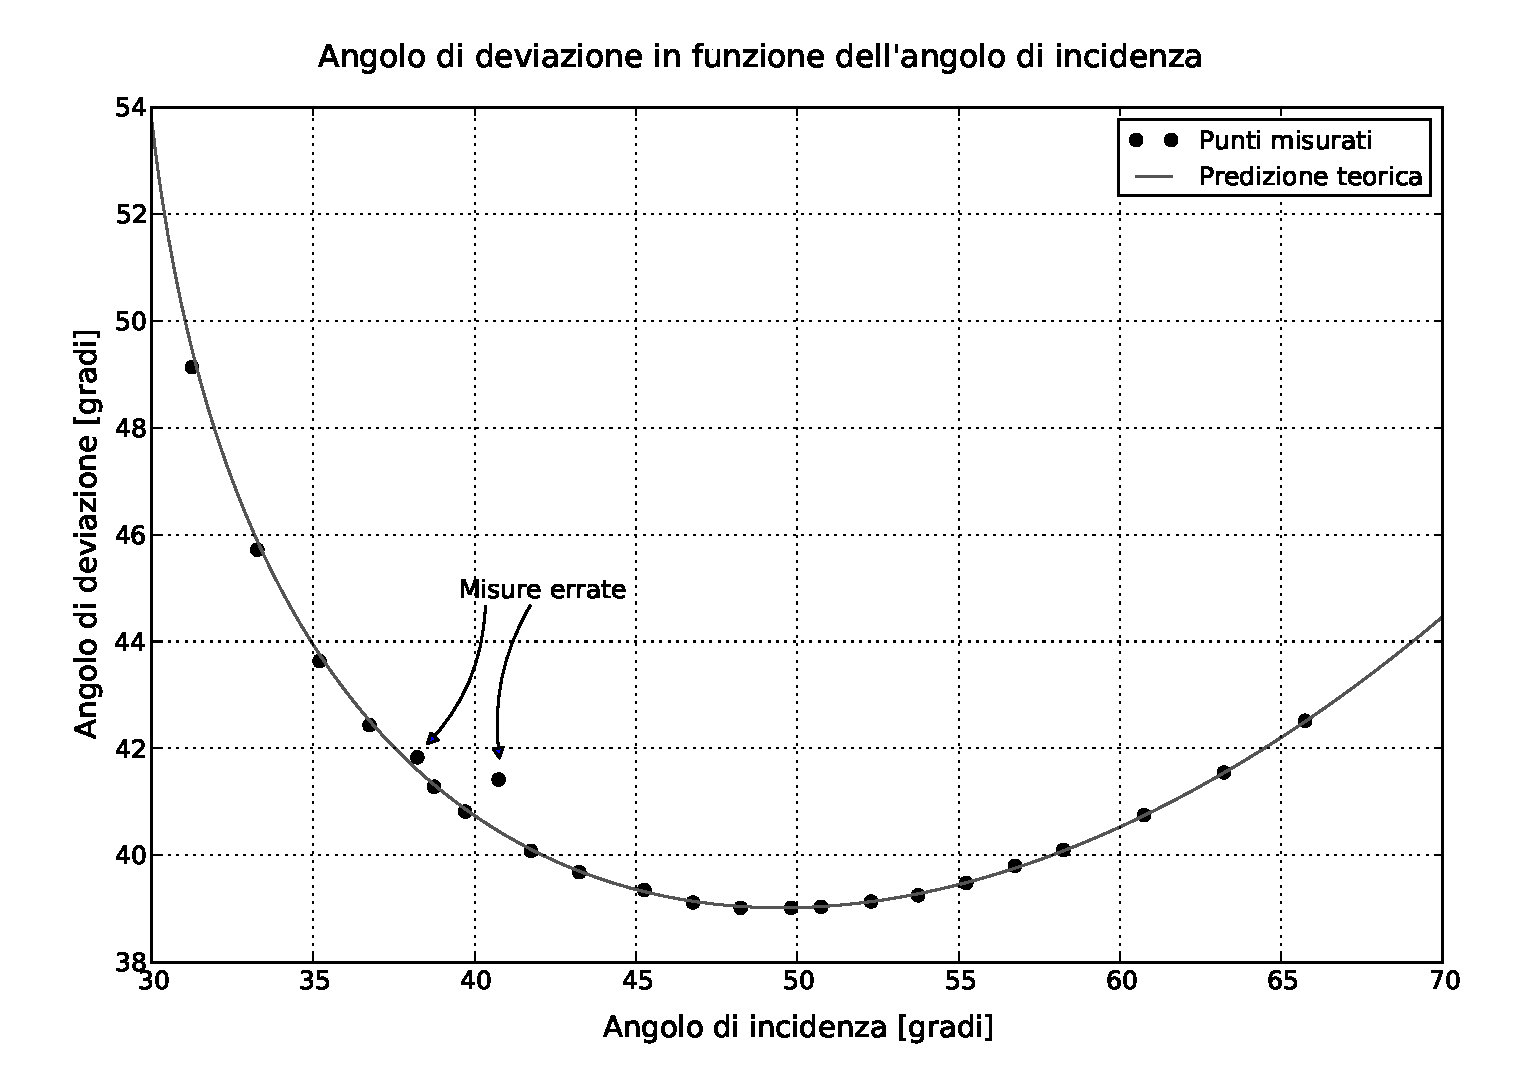
\includegraphics[width=16cm]{graph.pdf}
    \caption{Il grafico mostra i punti che abbiamo raccolto assieme ad un plot della legge (\ref{eq:brutta}). I dati concordano
    molto bene con la curva teorica, sebbene ci siano due punti errati, sicuramente dovuti ad errori nelle misure. L'errore di
    risoluzione è piccolo e non è mostrato in figura, in quanto le barre d'errore sono invisibili.}
    \label{fig:dev}
\end{figure}
